\documentclass[14pt]{extarticle}

\let\Overrightarrow\overrightarrow
\let\vecarrow\overrightarrow

%other%
\usepackage{graphicx}
\usepackage{float}
\usepackage[margin=0.7in]{geometry}
\usepackage{caption}
\usepackage{csquotes}
\usepackage[export]{adjustbox}
\usepackage{wrapfig}
\usepackage{setspace}
\usepackage{anyfontsize}
\usepackage{titlesec}
\titleformat{\section}{\normalfont\fontsize{20}{20}\bfseries}{\thesection}{1em}{}
\titleformat{\subsection}{\normalfont\fontsize{17}{20}\bfseries}{\thesubsection}{0.1em}{}
\usepackage{relsize}
\usepackage{indentfirst}
\usepackage{lipsum}
%other%


%math%
\usepackage[fleqn]{amsmath}
\usepackage{amsthm}
\usepackage{nccmath}
\usepackage{amsmath}
\usepackage{amssymb}
\usepackage{mathtools}
%\usepackage{unicode-math}
%\newtheorem*{}{\textup{Лемма}}
\newtheorem*{theorem}{\normalfont\fontsize{15}{15}\textup{Теорема}}
\newtheorem*{remark}{\textup{Комментарий}}
%\renewcommand\qedsymbol{$\blacksquare$}
%\usepackage{parski}
\renewenvironment{proof}
    {\noindent \textit{Доказательство.}\\
	\indent $\square$}
	{ $\blacksquare$\\ }

\newenvironment{solution}
	{\noindent\textbf{Решение.}}


\renewenvironment{remark}
    {\noindent\textbf{Комментарий.}}

\usepackage{tikz}
   \usetikzlibrary{calc}

\newcommand{\arc}[0]{
   \tikz [baseline = (N.base), every node/.style={}] {
	  \node [inner sep = 0pt] (N){}; %{$#0$};
      \draw [line width = 0.8pt] plot [smooth, tension=1.3] coordinates {
         ($(N.north west) + (-1.5ex,0.6ex+0.4ex)$)
         ($(N.north)      + (-0.75ex,0+0.4ex)$)
         ($(N.north east) + (0ex,0.6ex+0.4ex)$)
      };
   }
}

\renewenvironment{rcases}
  {\left.\begin{aligned}}
  {\end{aligned}\right\rbrace}

\DeclarePairedDelimiter\abs{\lvert}{\rvert}
\DeclarePairedDelimiter\norm{\lVert}{\rVert}

%\newcounter{example}[section]
\newenvironment{example}[1]{\noindent \textbf{Пример #1.}}
%\newcommand{\mathleft}{\mathindent0pt}
%{\@fleqntrue}
%\@mathmargin0pt}
%math%

%fonts%
\usepackage[russian]{babel}
\usepackage{polyglossia}
\setdefaultlanguage[spelling=modern]{russian}
%\setotherlanguage{english}
\setmainfont{CMU Serif}
\setsansfont{CMU Sans Serif}
\setmonofont{CMU Typewriter Text}  
%\setmathfont{Latin Modern Math}

\usepackage{unicode-math}
%\usepackage{fontspec}
\setmathfont{Latin Modern Math}

%fonts%


\begin{document}


\begin{center}
%\centering
	\textbf{\fontsize{23}{30}\selectfont Конкурентные прямые.}
\end{center}


В этом разделе мы рассмотрим одну из самых встречающихся тем 
в олимпиадной геометрии (планиметрии). Это целый класс
задач, в которых требуется доказать, что какие-то
прямые пересекаются в одной точке (или параллельны), такие прямые ещё называют
\textit{конкурентными}. Как правило их три, но может быть и больше.
В данном разделе мы ограничимся рассмотрением примеров,
где в основном фигурируют только три прямые.\\


\section*{Методы решения задач}

\subsection{Метод масс}
Для начала введем несколько базовых понятий.

\noindent \textit{\textbf{Материальная точка}} --- точка, которой 
\textquote{приписана} некоторая масса.

\noindent \textit{\textbf{Моментом}} материальной точки $A(m)$ относительно 
точки $Z$ называют вектор $m \, \Overrightarrow{ZA_{\,}}$.

\noindent Точка $Z$ называется \textit{\textbf{центром масс}} системы материальных 
точек\\
$A_1(m_1), \, A_2(m_2), \, ... \, , \, A_n(m_n)$, 
если $\mathlarger{\sum_{i=1}^{n} m_i \, \Overrightarrow{ZA_i} = \vec{0}}$.


\begin{theorem}[о существовании центра масс]
	Центр масс произвольной системы $A_1(m_1), \, ... \, ,A_n(m_n)$
	всегда существует, если $\mathlarger{\sum_{i=1}^{n} m_i \ne 0}$.
\end{theorem}

\begin{proof}
	Рассмотрим произвольную точку $X$. Тогда для любой  точки
	плоскости $O$ имеет место равенство $\mathlarger{\sum_{i=1}^{n}
	m_i \, (\vecarrow{XA_i} - \vecarrow{OX_{\, \,}}) = \sum_{i=1}^{n} 
	m_i \, \vecarrow{OA_i}}$. Тогда, чтобы точка $O$ была 
	\textit{центром масс} системы, должно выполняться равенство
	$\mathlarger{\sum_{i=1}^{n} 
	m_i \, \vecarrow{OA_i}} = \vec{0}$ $\iff \mathlarger{\sum_{i=1}^{n} m_i \,
	(\vecarrow{XA_i} - \vecarrow{OX_{\, \,}}) = \vec{0} \iff 
    \vecarrow{XO_{\;}} = \frac{\sum m_i \,
	\vecarrow{XA_i}}{\sum m_i}}$. То есть \\\onehalfspacing\\ утверждение
	о существовании \textit{центра масс} свелось к утверждению, что существует
	вектор $\vecarrow{XO_{\;}}$, заданный соответствующим соотношением, а он,
	понятное дело, существует. 
\end{proof}

\begin{remark}
	{\setstretch{1.5}
    Если условие $\mathlarger{\sum_{i=1}^{n} m_i \ne 0}$ не выполняется,
	то величина \\
	$\mathlarger{|\vecarrow{XO_{\;}}| = \abs[\bigg]{\frac{\sum m_i \,
	\vecarrow{XA_i}}{\sum m_i}}}$  не имеет смысла, поэтому это
	ограничение на сумму масс существенно.\par
    }
\end{remark}

\begin{theorem}[о единственности центра масс]
    Если центр масс системы $A_1(m_1), \\  \, ... \, ,A_n(m_n)$
	существует, то он единственен.
\end{theorem}

\begin{proof}
От противного. Пусть существуют два различных центра масс $Z$ и $Z'$.
Тогда по определению имеем: $\mathlarger{\sum_{i=1}^{n} m_i \, \vecarrow{ZA_i}
= \vec{0},}$ \quad $\mathlarger{\sum_{i=1}^{n} m_i \, \vecarrow{Z'A_i}} = \vec{0}. 
\implies$\\
$\implies \mathlarger{\sum_{i=1}^{n} m_i \, \vecarrow{ZZ'_{\;\:\,}}} = \vec{0}$
$\iff \mathlarger{\vecarrow{ZZ'_{\;\:\,}} \sum_{i=1}^{n} m_i} = \vec{0}$. 
$\iff \vecarrow{ZZ'_{\;\:\,}} = \vec{0}$ (последний переход верен, 
так как центр масс существует, то есть
$\mathlarger{\sum_{i=1}^{n} m_i \ne 0}$) $\iff Z = Z'$, что противоречит
предположению, что точки $Z$ и $Z'$ различны. $\implies$ центр масс $Z$
единственен.
\end{proof}

\noindent Далее будем считать, что $\mathlarger{\sum_{i=1}^{n} m_i \ne 0}$.

\begin{theorem}[о группировке масс]
Пусть есть система материальных точек $A_1(m_1),  \, A_2(m_2), \, ... \, ,
\, A_n(m_n), \, B_1(k_1), \, B_2(k_2), \, ... \, , \, B_l(k_l)$, 
	и подсистема $A_1(m_1), \\ \, A_2(m_2), \, ... \, , 
	\, A_n(m_n)$ имеет центр масс $W$.
Назовем редуцированной системой систему $W(m_1 + ... + m_n), B_1(k_1),
\, B_2(k_2), \, ... \, , \, B_l(k_l)$. Тогда исходная система имеет ц.м. $Z$
в том и только том случае, когда редуцированная система имеет ц.м. $Z$.
\end{theorem}


%$\mathlarger{M = \sum_{i=1}^{l+n} m_i}$,\\
%$\mathlarger{A = \sum_{j=1}^{n} m_j}$.

\begin{proof}
Согласно \textit{определению} центра масс, надо доказать равносильность\\
$\mathlarger{\sum_{i=1}^{n} m_i \, \Overrightarrow{ZA_i} \: + 
\sum_{j=1}^{l} k_j \, \Overrightarrow{ZB_j}} = \vec{0} \iff 
\mathlarger{\sum_{j=1}^{l} k_j \, \Overrightarrow{ZB_j} + 
	 \sum_{i=1}^{n} m_i \, \Overrightarrow{ZW_{\: \,}}} = \vec{0}$.
%\noindent 
То есть надо показать равенство:
$\mathlarger{\sum_{i=1}^{n} m_i \, \Overrightarrow{ZA_i} = 
\Overrightarrow{ZW_{\: \,}} \sum_{i=1}^{n} m_i}$ $\iff$   
$\mathlarger{\sum_{i=1}^{n}
m_i \, (\Overrightarrow{ZA_i} - \Overrightarrow{ZW_{\: \,}})} = \vec{0}$ 
$\iff \mathlarger{\sum_{i=1}^{n}
m_i \, \Overrightarrow{WA_i}} = \vec{0}$, что верно в силу того, что $W$ ---
центр масс подсистемы $A_1(m_1), \, A_2(m_2), \, ... \, , \, A_n(m_n)$.
\end{proof}


Метод масс широко используется при доказательстве теорем и задач на
конкурентность прямых, причем их может быть любое количество, а ключевым 
элементом решения является именно \textit{теорема о группировке масс}. 


\subsection{Теорема Чевы} 

\indent Один из самых мощных методов доказательства того, что три прямые 
проходят через одну точку или параллельны. 
Приведем ниже доказательство через \textit{метод масс}.
С другими доказательствами этой теоремы (через площадь, подобие и др.) 
вы можете ознакомится в других источниках, например, в книге Я. П. Понарина
\textquote{Элементарная геометрия. Том 1}.


\begin{theorem}[Чевы]
	Пусть на прямых $AB$, $BC$, $CA$, определяющих
    треугольник ABC, даны точки $C_1$, $A_1$, $B_1$. Для того, чтобы прямые
    $AA_1$ , $BB_1$, $CC_1$ пересекались в одной точке или были параллельными,
    необходимо и достаточно, чтобы
	
	\begin{ceqn}
	\[
    \dfrac{\Overrightarrow{AB_1}}{\Overrightarrow{B_1C_{\, \,}}} \cdot 
	\dfrac{\Overrightarrow{CA_1}}
	{\Overrightarrow{A_1B_{\:}}} \cdot \dfrac{\Overrightarrow{BC_1}}
	{\Overrightarrow{C_1A_{\,}}} = 1
	\]
    \end{ceqn}

\end{theorem}


\begin{wrapfigure}{r}{9cm}
	\hspace{-0.3cm}
	\vspace{-0.6cm}
	\fcolorbox{white}{white}{
		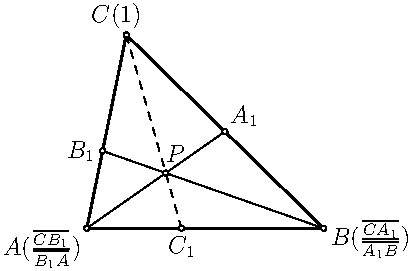
\includegraphics[width=9cm]{./img/ceva.pdf}}
	\vspace{-1cm}
\end{wrapfigure}

\begin{proof}
    Пусть $AA_1 \cap BB_1 = P$, $CP \cap AB = C_1$. 
	Поместим массы $1, \: \frac{\overline{CA_1}}{\vphantom
	{\overline{AB'}}\overline{A_1B}}, 
	\: \frac{\overline{CB_1}}{\vphantom
	{\overline{AB'}}\overline{B_1A}}$ (здесь за $\overline{v}$
	обозначается вектор $v$)
	в точки $C, \: B, \: A$ соответственно. Тогда центр масс точек
	$B$ и $C$ находится в $A_1$, а значит, по теореме о группировке
	масс, центр масс вершин $\triangle ABC$ лежит на прямой $AA_1$.
	Аналогично получаем, что он лежит и на $BB_1$. Следовательно,
	$P$ --- центр масс вершин $\triangle ABC$, согласно 
	\textit{теореме о единственности центра масс}. 
	Так как $P \in CC_1$, центр масс точек $B$ и $A$ находится в $C_1$.
	Из этого следует, что $\dfrac{\Overrightarrow{CB_1}}
	{\Overrightarrow{B_1A_{\,}}} \cdot \Overrightarrow{C_1A_{\,}} +
	\Overrightarrow{C_1B_{\:}} \cdot
	\dfrac{\Overrightarrow{CA_1}}{\Overrightarrow{A_1B_{\:}}} = \vec{0}$
    $\iff$ 
	$
	\dfrac{\Overrightarrow{AB_1}}{\Overrightarrow{B_1C_{\, \,}}} \cdot 
	\dfrac{\Overrightarrow{CA_1}}
	{\Overrightarrow{A_1B_{\:}}} \cdot \dfrac{\Overrightarrow{BC_1}}
	{\Overrightarrow{C_1A_{\,}}} = 1$.
	Мы доказали сразу и \textit{необходимость}, и \textit{достаточность},
	потому что полученное выражение является критерием пренадлежности точки
	$P$ прямой $CC_1$, то есть
	т\\ого, что все три чевианы проходят через одну точку.\\
    
	Пусть теперь  прямые $AA_1$ и $BB_1$ параллельны. Докажем, что 
	тогда прямая $CC_1$ им параллельна. От противного. Пусть
	$CC_1 \cap BB_1 = P$, тогда, аналогично доказанному выше, получаем, что
	через точку $P$ проходит прямая $AA_1$, так как $P$ --- центр масс
	вершин $\triangle ABC$, а мы доказали, что если две прямые
	через него проходят, то и третья тоже через него проходит,
	но $P \in AA_1$  противоречит предположению
	$AA_1 \parallel BB_1. \implies CC_1 \parallel BB_1 \parallel AA_1$.
\end{proof}

Формулу теоремы Чевы несложно запомнить, если при записи отношений
пользоваться правилом \textquote{\textit{в числителе: вектор от текущей вершины
до основания чевианы, для которого еще не записано отношение,
а в знаменателе: вектор от текущего основания чевианы до другой вершины
на данной прямой, содержащей основание чевианы и предыдущую вершину}}.
То есть мы обходим треугольник по или против часовой стрелки и записываем
отношения по данному правилу.
%$\blacksquare$ \\
%%\begin{remark}
%%\textup{
%%Доказательство остается верным, если точки $A_1, \: B_1, \: C_1$ лежат
%%так, что $AA_1 \parallel BB_1$, тогда ввиду следующих
%%соображений вышеописанные рассуждения остаются верными. Пусть $AA_1
%%\parallel BB_1$, тогда говорят, что $AA_1 \cap BB_1 = P$, где $P$ --- т.н. 
%%\textit{бесконечно удаленная точка}. Тогда вышеописанное тождество остается
%%критерием пренадлежности точки $P$ прямой $CC_1$, т.к. если $P \in CC_1$, то 
%%по определению \textit{бесконечно удаленной точки} --- $CC_1 \parallel BB_1
%%\parallel AA_1$, а если $CC_1 \nparallel AA_1$, то так же по определению
%%\textit{бесконечно удаленной точки} --- $P \notin CC_1$. %С геометрической же точки зрения это означает
%%}
%%\end{remark}


%\end{proof}



\noindent \textbf{Примечание}


\begin{wrapfigure}{r}{8cm}
	\hspace{-1cm}
	%\vspace{-2cm}
	\fcolorbox{white}{white}{
		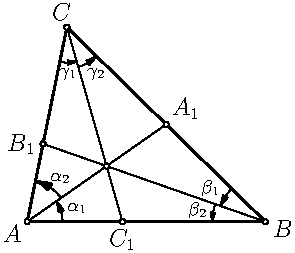
\includegraphics[width=6.5cm, right]{./img/ceva_trig.pdf}}
	%\vspace{-1.5cm}
\end{wrapfigure}

\noindent \textbf{\small Тригонометрическая (угловая) форма теоремы Чевы}.\\
Если ввести в рассмотрение \textit{ориентированные} углы $\alpha_1 = \angle BAA_1$, 
$\alpha_2 = \angle A_1AC$, $\gamma_1 = \angle ACC_1$, $\gamma_2 = \angle C_1CB$,
$\beta_1 = \angle CBB_1$, $\beta_2 = \angle B_1BA$, то соотношение теоремы
Чевы можно представить в эквивалентном виде через синусы этих углов, а именно


%\begin{flalign*}
{\setlength{\mathindent}{2.5cm}
\begin{equation*}
\dfrac{\sin \alpha_1}{\sin \alpha_2} \cdot 
	\dfrac{\sin \gamma_1}{\sin \gamma_2} 
\cdot \dfrac{\sin \beta_1}{\sin \beta_2} = 1 
\end{equation*}}
%\end{flalign*}
%\vspace{5mm}
	

    %\centerin

Предлагаем читателю доказать данное  утверждение самостоятельно, это 
будет хорошим упражнением.
%Если возникнут трудности, то можно обратиться к \textbf{примеру 1}, там есть
%соображения, которые могут помочь вам при доказательстве этой теоремы.

\subsection{Принадлежность точки пересечения двух прямых третьей}

\begin{wrapfigure}{r}{7cm}

\vspace{0cm}
%\hspace{1cm}
%\centering
	\fcolorbox{white}{white}{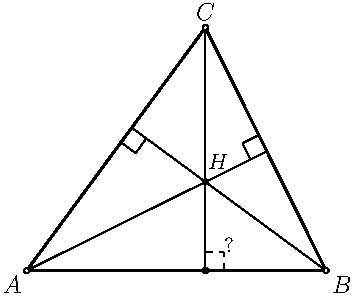
\includegraphics[width=7cm]{./img/orthicproof.pdf}}
\vspace{-1cm}
\end{wrapfigure}

Можно попробовать доказать, что точка пересечения каких-то двух прямых из трех
принадлежит третьей прямой. Классическим примером является доказательство
того, что высоты, медианы и биссекрисы треугольника пересекаются в одной точке.
С помощью данного метода иногда так же легко доказываются и более сложные вещи,
например, то, что \textit{радикальные оси} трех окружностей конкурентны. 
Точнее, таким способом можно доказать, что в \textit{нетривиальном} случае они 
проходят через одну точку, а \textit{тривиальный} случай можно разобрать
отдельно. Этот метод можно по-разному использовать, например, доказать
конкурентность высот треугольника можно исходя из следующих соображений: 
\textit{проведем две высоты и третью прямую, проходящую через точку пересечения
двух высот и через третью вершину треугольника, а потом докажем, что это и будет
искомая высота}.




\subsection{Преобразование плоскости}
Можно сделать \textit{преобразование плоскости} $f$, отображающее плоскость на себя,
которое переводит исходные прямые \(a, \, b, \, c\), про которые нам нужно доказать,
что они конкурентны, в некоторые прямые \(a', \, b', \, c'\), причем,
\(a \parallel a', \, b \parallel b', \, c \parallel c'\).
%, отображающее плоскость в себя,
%которое переводит кажду прямую в
%параллельную ей прямую(\textit{аффинное преобразование}), 
Тогда, если их образы \(a', \, b', \, c'\) конкурентны, то и исходные
прямые были таковыми.

Докажем равносильность конкурентности образов прямых и исходных прямых.
%Пусть исходные прямые --- $a, b, c$

\textit{Необходимость.}

Пусть $a \cap b \cap c = M$; $\forall i \in \{a, \: b, \: c\} \mathpunct{:} f(i) = i'$ 
и $f(M) = M'$. Заметим, что $\forall i \in \{a, \: b, \: c\} \mathpunct{:} M \in i 
\Rightarrow M' \in f(i) \implies M' \in a', \:  b', \: c'$. 

Если же $a \parallel b \parallel c$, то, т.к. $f$ переводит \(a, \, b, \, c\)
в параллельные им прямые, имеем следующее: \(a \parallel b \parallel c \implies
f^{-1}(a) \parallel f^{-1}(b) \parallel f^{-1}(c) \iff a' \parallel b' \parallel
c'\).\\


\textit{Достаточность.}

Пусть $a', \: b', \: c'$ --- образы прямых $a, \: b, \: c$ соответственно при
преобразовании плоскости $f$, $a' \cap b' \cap c' = M'$,
$f^{-1}(M') = M$. Тогда 
\begin{ceqn}
\[
\begin{rcases}
	f^{-1}(a') &= a\\
	f^{-1}(b') &= b\\
	f^{-1}(c') &= c\\
	f^{-1}(M') &= M\\
	M' \in a', \: &b' , \: c' \\
\end{rcases}
\text{$\Rightarrow M \in a,\: b, \: c$}
\]
\end{ceqn}

%Если же $a' \parallel b' \parallel c'$, то т.к. $f$ переводит параллельные
%прямые в параллельные $f^{-1}(a') \parallel f^{-1}(b') \parallel f^{-1}(c')
%\iff a \parallel b \parallel c$.\\


Если же $a' \parallel b' \parallel c'$, то, т.к. $f$ переводит \(a, \, b, \, c\)
в параллельные им прямые и \(f\) --- \textit{биективное} преобразование плоскости, имеем
следующее: \(a' \parallel b' \parallel c' \implies
f^{-1}(a') \parallel f^{-1}(b') \parallel f^{-1}(c') \iff a \parallel b \parallel
c\).\\

%Потому что точка $M'$ (точка пересечения образов прямых)
%единствененa и принадлежит одновременно всем образам $\Rightarrow$ 
%$M$ (прообраз $M'$) принадлежит всем прообразам. А если исходные прямые были
%попарно параллельны, то и их образы были 
\textit{(Данный метод применим не только для случая 
$n=3$, но и для любого количества прямых)} 

\begin{remark}
	Если требуется только, чтобы прямые \(a, \, b, \, c\) пересекались в одной
    точке, то достаточно, чтобы $f$ переводило \(a, \, b, \, c\) в любые прямые.
    В таком случае пересечение прямых \(a, \, b, \, c\) в одной точке,
    по вышеописанным причинам, также сохраняется.
\end{remark}

\subsection{Известные прямые}
\indent Посмотреть, может быть это какие-то известные три прямые, про
которые вы знаете, что они конкурентны, например, это могут быть 
три прямые, которые являются радикальными осями каких-то окружностей или
медианами/бисcектрисами/высотами, или просто конкурентными чевианами
в каком-нибудь треугольнике. Можно также начать действовать с конца. То есть
в предположении, что утверждение доказано выявить какие-нибудь полезные 
\textit{признаки} картинки и попытаться ими воспользоваться. Таким образом можно 
свести исходную задачу к равенству углов, подобию/гомотетичности треугольника и
т.п., и постараться доказать уже новое утверждение.


\subsection{Изогонали и изогональное сопряжение}
В продолжение предыдущего подраздела про известные прямые рассмотрим такие
прямые, которые называют \textit{изогоналями}.\\

\noindent\textbf{Определение.} Прямые \(AP\) и \(AQ\) называются 
\textbf{\textit{изогоналями}} относительно данного угла \(BAC\),
если \(\angle PAB = \angle QAC\). (Что, очевидно, эквивалентно следующему:
\(AP\) и \(AQ\) симметричны относительно биссектрисы угла \(BAC\)).


\begin{theorem}[\textit{основная теорема об изогоналях}]
Пусть имеются прямые \(a\), \(b\), \(c\), проходящие через точки \(A,\, B,
\, C\) соответственно. Тогда \(a, \, b, \, c\)  конкурентны \(\iff\)
\(a', \, b', \, c'\) конкурентны, 
где \(a'\) и \(a\); \(b'\) и \(b\); \(c'\) и \(c\) --- изогонали
относительно углов \(A,\, B, \, C\) cоответственно.
\end{theorem}

%\(a \cap b \cap c = p  \iff a' \cap b' \cap c'
%= p'\), \(a \parallel b \parallel c \iff a' \parallel b' \parallel c'\),

\begin{proof}
Докажем сначала, что из конкуретности прямых \(a, \, b, \, c\)
следует конкурентность прямых \(a', \, b', \, c'\).

Пусть \(\angle PCB = \gamma\), \( \angle BAP = \alpha\), \\
\(\angle CBP = \beta\). Пусть так же \(\angle P'CP = \gamma'\), \par
\begin{wrapfigure}{r}{87mm}
    \vspace{-2cm}
    \fcolorbox{white}{white}{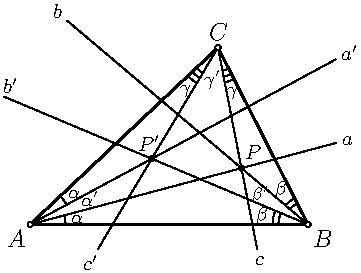
\includegraphics[width=87mm]{./img/isogonal.pdf}}
	%\vspace{-1cm}
\end{wrapfigure}
\noindent\(\angle PAP' = \alpha'\), \(\angle PBP' = \beta'\) (здесь все углы
ориентированные). Тогда для прямых  \(a, \, b, \, c\) из угловой теореме
Чевы имеем следующее:
\[
\frac{\sin \alpha}{\sin(\alpha + \alpha ')} \cdot
\frac{\sin(\gamma + \gamma ')}{\sin \gamma} \cdot
\frac{\sin \beta}{\sin(\beta + \beta ')} 
 = 1
\]

\noindent А теперь заметим, что 
\[
\frac{\sin(\alpha + \alpha ')}{\sin \alpha} \cdot
\frac{\sin \gamma}{\sin(\gamma + \gamma ')} \cdot
\frac{\sin(\beta + \beta ')}{\sin \beta} 
 = 1
\]
Но ведь это --- выражение угловой формы теоремы Чевы для прямых
\(a'\), \(b'\), \(c'\). А значит, согласно угловой теореме Чевы, 
\(a'\), \(b'\), \(c'\) конкурентны.
%\(a' \cap b' \cap c' = p'\).
Обратное следствие доказывается аналогично.
\end{proof}
\noindent {\normalfont\fontsize{14}{14}\textbf{\textit{Примечание.}}}
 Точки \(P\) и \(P'\) называют \textit{изогонально сопряжёнными}.\\

\noindent Приведем ниже, как дополнение, интересный факт,
доказательство которого Вы можете найти, например, в статье
\textquote{Теорема об изогоналях} А.Куликовой и Д.Прокопенко.

%\noindent {\normalfont\fontsize{14}{14}\textbf{Теорема об изогоналях}}. 
\begin{theorem}
Пусть \(OB\) и \(OC\) --- изогонали угла \(AOD\). Прямые
\(AC\) и \(BD\) пересекаются в точке \(Q\), прямые \(AB\) и \(CD\)
--- в точке \(P\). Тогда \(OP\) и \(OQ\) --- также изогонали 
относительно угла \(AOD\).\\
\end{theorem}


\subsection{Теорема Дезарга}
\textbf{<ТУТ БУДЕТ ТЕОРЕМА ДЕЗАРГА>}\\

%\noindent 
Понятное дело, что это далеко не самый полный список методов
доказательства таких задач. Цель данного раздела --- показать, в каких
направлениях можно
продвигаться в задачах такого типа, если не понятно, как начать действовать. 
%\newpage


\section*{Примеры}
Давайте рассмотрим теперь применение данных методов при решение
конкретных задач.\\

%\noindent \textbf{Пример 1}.
\begin{example}{1}
В треугольнике $ABC$ $AL_a$, $BL_b$, $CL_c$
--- биссектрисы, $K_a$ --- точка пересечения касательных к описанной
окружности в вершинах $B$ и $C$, $K_b$, $K_c$ определены
аналогично. Докажите, что прямые $K_a L_a$, $K_b L_b$ и $K_c L_c$
пересекаются в одной точке.
\textit{(Заочный тур oлимпиады им. И.Ф.Шарыгина 2019)}\\
\end{example}


%\hfill \break

\begin{solution}
    
	%\textit{Инверсия} здесь явно не поможет, потому что данные прямые не 
	%проходят через центр какой-нибудь \textquote{\textit{удобной}} 
	%окружности, и поэтому вообще перейдут в окружности, следовательно нам
	%ничего доказать не удастся. 

    Чтобы понять, какой из вышеописанных методов поможет в решении
    данной задаче, обратимся к рисунку (см. рис. 1). 
	Из известных преобразований плоскости тут мало что может помочь.
	Скажем, используя, \textit{поворот}, или \textit{осевую симметрию},
	или \textit{параллельный перенос} --- не совсем понятно относительно
	чего производить
	эти преобразования, и что куда при них перейдет.
    Использование \textit{гомотетии} также не 
	кажется, по крайней мере на первый взгляд, осмысленным, т.к.
	мы ничего не можем сказать про отношения отрезков 
	(кроме, разве что, в $\triangle ABC$), поэтому не поймем что куда 
	перейдет. Остается последний вариант --- теорема Чевы. На первый
	взгляд её использование здесь вам может показаться неуместным, но
	не торопитесь с выводами. Итак, давайте разбираться, как же
	все-таки здесь использовать теорему Чевы. 

	\begin{figure}[H]
	
	%\vspace{-1cm}
	\hspace{1cm}
	%\centering
	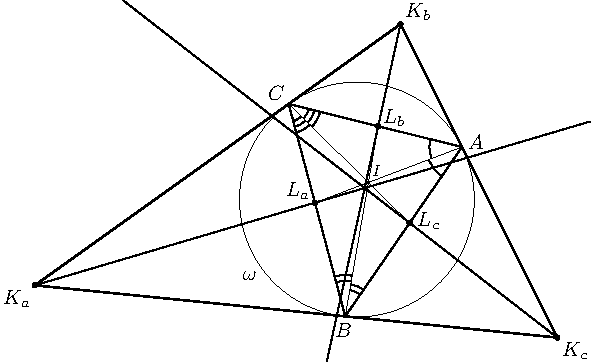
\includegraphics[width=15cm]{./img/sharygin_19_2019.pdf}
	\caption{}
	\end{figure}

    Как мы помним, в теореме Чевы нам нужно, чтобы произведение отношений
	соответствующих направленных отрезков было равно 1, тогда и только тогда
	прямые пересекутся в одной точке. Здесь отношения таких отрезков 
	считать неудобно, поэтому давайте лучше постараемся
	все-таки понять что-то про расположение данных прямых. 
	Единственное, отношение чего мы знаем --- отношения отрезков, содержащие
	основания биссекрис $\triangle ABC$. Было бы хорошо понять что-нибудь 
	про расположение самих прямых, например, углы относительно сторон 
	$\triangle K_a K_b K_c$. Давайте отдельно перерисуем фрагмент рисунка, 
	содержащий одну из трех прямых ($K_a L_a$, $K_b L_b$, $K_c L_c$),
	и исследуем его.


	\begin{figure}[H]
	
	%\vspace{-1cm}
	%\hspace{6cm}
	\centering
	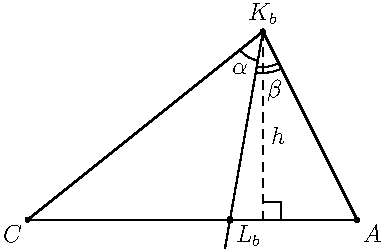
\includegraphics[height=6cm]{./img/sharygin_19_2019_2.pdf}
	\caption{}
	\end{figure}

	{\setstretch{1.6} Попробуем как-то привязаться к углам \(\alpha\)
    и \(\beta\), зная отношение $\dfrac{CL_b}{L_bA}$. 
	Давайте вспомним, что площадь треугольника
	можно посчитать как полупроизведение сторон на синус угла между ними.
	То есть \hspace{0mm} $S_{CK_bL_b} = \dfrac{CK_b 
	\cdot K_bL_b \cdot \sin \alpha}{2}$.
	Аналогично $S_{AK_bL_b} = \dfrac{K_bL_b \cdot K_bA \cdot \sin \beta}{2}$.
	Откуда получаем $\dfrac{S_{CK_bL_b}}{S_{AK_bL_b}} = \dfrac{CK_b \cdot
	\sin \alpha}{K_bA \cdot \sin \beta}$.
	С другой стороны 
	$S_{AK_bL_b} = \dfrac{h \cdot L_bA}{2}$ \hspace{0mm} и 
	\hspace{0mm} $S_{CK_bL_b} = \dfrac{h \cdot L_bC}{2}$. \par }
	
	{\setstretch{1.8} Тогда \hspace{0mm} $\dfrac{S_{CK_bL_b}}{S_{AK_bL_b}} = 
	\dfrac{L_bC}{L_bA}$. И окончательно $\dfrac{S_{CK_bL_b}}{S_{AK_bL_b}} =
	\dfrac{CK_b \cdot \sin \alpha}{K_bA \cdot \sin \beta} = 
	\dfrac{L_bC}{L_bA}$.
	
    Но ведь  $K_bC$ и $K_bA$ --- это отрезки касательных к
	окружности $\omega$ из одной \par} \noindent точки $\Rightarrow 
	K_bC = K_bA$. \\ \indent В итоге полученное выражение преобретает вид
	$\dfrac{\sin \alpha}{\sin \beta} = \dfrac{L_bC}{L_bA}$.

	Мы видим отношение двух синусов, что наталкивает нас на мысль о том, что
	на самом деле мы будем использовать \textquote{\textit{угловую}} форму
	теоремы Чевы.

	Теперь остается лишь написать схожее отношение для всех трех прямых 
	и перемножить.\\

    
	$\dfrac{\sin \angle K_cK_aL_a}{\sin \angle L_aK_aK_b} \cdot
	\dfrac{\sin \angle K_aK_bL_b} {\sin \angle L_bK_bK_c} \cdot
	\dfrac{\sin \angle K_bK_cL_c}{\sin \angle L_cK_cK_a} = 
	\dfrac{BL_a}{L_aC} \cdot \dfrac{CL_b}{L_bA} \cdot \dfrac{AL_c}{L_cB} = 1$ \\
	
	(последнее равенство верно, т.к. биссектрисы пересекаются в одной точке)

	Тогда, согласно \textquote{\textit{угловой}} форме теоремы Чевы,
	прямые $K_aL_a, K_bL_b, K_cL_c$ пересекаются в одной точке. \vspace{2mm}

\end{solution}


\begin{remark}
	Вектора мы опустили, потому что основания бисcектрис всегда лежат
	на сторонах треугольника.
	Однако стоит отметить, что условие \textquote{$BL_b, AL_a, CL_c$ 
	--- биссектрисы}
	мы использовали, только когда считали отношение синусов
	соответствующих углов. То есть, вообще-то говоря,
    $BL_b, AL_a, CL_c$ могли быть любыми \textit{чевианами} в $\triangle ABC$,
	основания которых лежат на сторонах треугольника,
    и которые  пересекаются в одной точке.\\
\end{remark}

\begin{example}{2}
В треугольнике $ABC$ $AH_1$ и $BH_2$ ---  высоты; касательная к описанной
окружности в точке $A$ пересекает $BC$ в точке $S_1$, а касательная в точке
$B$ пересекает $AC$ в точке $S_2$; $T_1$ и $T_2$ --- середины отрезков
$AS_1$ и $BS_2$. Докажите, что $T_1T_2$, $AB$ и $H_1H_2$
пересекаются в одной точке.
\textit{(Заочный тур oлимпиады им. И.Ф.Шарыгина 2019)}\\
\end{example}

\begin{solution}
На первый взгляд задача кажется достаточно трудной, однако можно снова
обратиться к списку вышеописанных методов и выбрать нам подходящий, 
как мы делали в предыдущем примере.\\
\end{solution}

\begin{example}{3}
Даны три окружности. Первая и вторая пересекаются в точках $A_0$ и $A_1$,
вторая и третья --- в точках $B_0$ и $B_1$, третья и первая --- в точках
$C_0$ и $C_1$. Пусть $O_{i,j,k}$ --- центр описанной окружности
треугольника $A_iB_jC_k$ . Через все пары точек	вида $O_{i,j,k}$
и $O_{1−i,1−j,1−k}$ провели прямые. Докажите, что эти 4 прямые пересекаются
в одной точке или параллельны.
\textit{(Заочный тур oлимпиады им. И.Ф.Шарыгина 2019)}\\
\end{example}

\begin{example}{4}
Каждая из окружностей \(S_1\), \(S_2\) и \(S_3\) касается внешним образом
окружности \(S\) (в точках \(A_1\), \(B_1\), \(C_1\) соответственно) и двух
сторон треугольника \(ABC\) (см. рис.). Докажите, что прямые \(AA_1\),
\(BB_1\), \(CC_1\) пересекаются в одной точке.
\end{example}


\section*{Задачи}
ТУТ БУДУТ ЗАДАЧИ ДЛЯ САМОСТОЯТЕЛЬНОГО РЕШЕНИЯ.

\section*{Подсказки}
ТУТ БУДУТ ПОДСКАЗКИ К ЗАДАЧАМ ДЛЯ САМОСТОЯТЕЛЬНОГО РЕШЕНИЯ.




\begin{thebibliography}{9}
\bibitem{ponarin}
Я. П. Понарин Элементарная геометрия Том 1

\bibitem{kulikovaprokopenko}
А.Куликова, Д.Прокопенко --- \textquote{Теорема об изогоналях} \\
\texttt{http://geometry.ru/articles/isogonal\_theorem\_kvant\_04\_05.pdf}

\end{thebibliography}



\end{document}
